%%%%%%%%%%%%%%%%%%%% author.tex %%%%%%%%%%%%%%%%%%%%%%%%%%%%%%%%%%%
%
% sample root file for your "contribution" to a contributed volume
%
% Use this file as a template for your own input.
%
%%%%%%%%%%%%%%%% Springer %%%%%%%%%%%%%%%%%%%%%%%%%%%%%%%%%%%%%%%%%


%% RECOMMENDED %%%%%%%%%%%%%%%%%%%%%%%%%%%%%%%%%%%%%%%%%%%%%%%%%%%
%\documentclass[graybox]{svmult}
%
%% choose options for [] as required from the list
%% in the Reference Guide
%
%\usepackage{mathptmx}       % selects Times Roman as basic font
%\usepackage{helvet}         % selects Helvetica as sans-serif font
%\usepackage{courier}        % selects Courier as typewriter font
%\usepackage{type1cm}        % activate if the above 3 fonts are
                             % not available on your system
%
%\usepackage{makeidx}         % allows index generation
%\usepackage{graphicx}        % standard LaTeX graphics tool
%                             % when including figure files
%\usepackage{multicol}        % used for the two-column index
%\usepackage[bottom]{footmisc}% places footnotes at page bottom
%
%% see the list of further useful packages
%% in the Reference Guide
%
%\makeindex             % used for the subject index
%                       % please use the style svind.ist with
%                       % your makeindex program
%
%%%%%%%%%%%%%%%%%%%%%%%%%%%%%%%%%%%%%%%%%%%%%%%%%%%%%%%%%%%%%%%%%%%%%%%%%%%%%%%%%%%%%%%%%%
%
%\begin{document}

\title{Buildings}
% Use \titlerunning{Short Title} for an abbreviated version of
% your contribution title if the original one is too long
\author{
    \textbf{Adam Zsarnóczay}
    \and Jack W. Baker}
\tocauthor{}
\authorrunning{Zsarnóczay and Baker}
% Use \authorrunning{Short Title} for an abbreviated version of
% your contribution title if the original one is too long
%\institute{Name of First Author \at Name, Address of Institute, %\email{name@email.address}
%\and Name of Second Author \at Name, Address of Institute %\email{name@email.address}}
%
% Use the package "url.sty" to avoid
% problems with special characters
% used in your e-mail or web address
%
\maketitle

Buildings are arguably the most important asset type when it comes to direct consequences of a natural disaster. A severely damaged or collapsed building may result in loss of life, injuries, and significant capital losses. Historically, two different approaches have been developed mostly in parallel for performance assessment of buildings (Figure \ref{fig:perf_PBEapproaches}):

\begin{itemize}
    \item Large-scale simulations of distributed building inventories required idealized, efficient models that provided sufficiently accurate performance estimates while limiting the computational workload to make the simulations feasible. The most popular example of such an approach is the HAZUS framework that has been developed for earthquake \citep{fema2018earthquaketechnical}, hurricane \citep{fema2018hurricaneuser}, and tsunami hazards \citep{fema2017tsunamitechnical}. HAZUS and similar methods typically take path I or II in Figure \ref{fig:perf_PBEapproaches} and estimate the consequences of a disaster using vulnerability or fragility functions that link the intensity of the natural hazard directly to measures of damage and losses at the building level. 
    \item The assessment of individual buildings has been moving from a holistic towards a component-based approach. Instead of trying to characterize the building damage as a whole, recent performance-based engineering methods disaggregate buildings into sets of components and apply separate models (i.e., functions) to estimate the damage and losses for each component. These methods require a detailed description of the building and its behavior under the natural hazard event which necessitates the simulation of building response following path III in Figure \ref{fig:perf_PBEapproaches}. In return, they provide high-resolution information about the damages and losses that allow better understanding of the building's performance. FEMA P-58 \citep{atc2018p-58-1} represents the state-of-the-art in high-fidelity seismic performance assessment for buildings. Researchers have recently been developing similar performance-based engineering methodologies for other hazards (e.g. \cite{barbato2013performancebased, ouyang2020performance, attary2017performancebased}).
\end{itemize}

The two approaches presented above were traditionally separated because neither the computational resources nor the detailed description of assets were available to apply to high-fidelity models and methods at a large scale. Recent advances in computational resources, data harvesting and processing (see Part \ref{part:cross}) already enable experimentation with bridging the gap between these methods and suggest that integrated multi-fidelity performance assessment of large asset portfolios will become available for researchers in the near future \citep{deierlein2020cloud}.

\begin{figure}[htb]
    \centering
    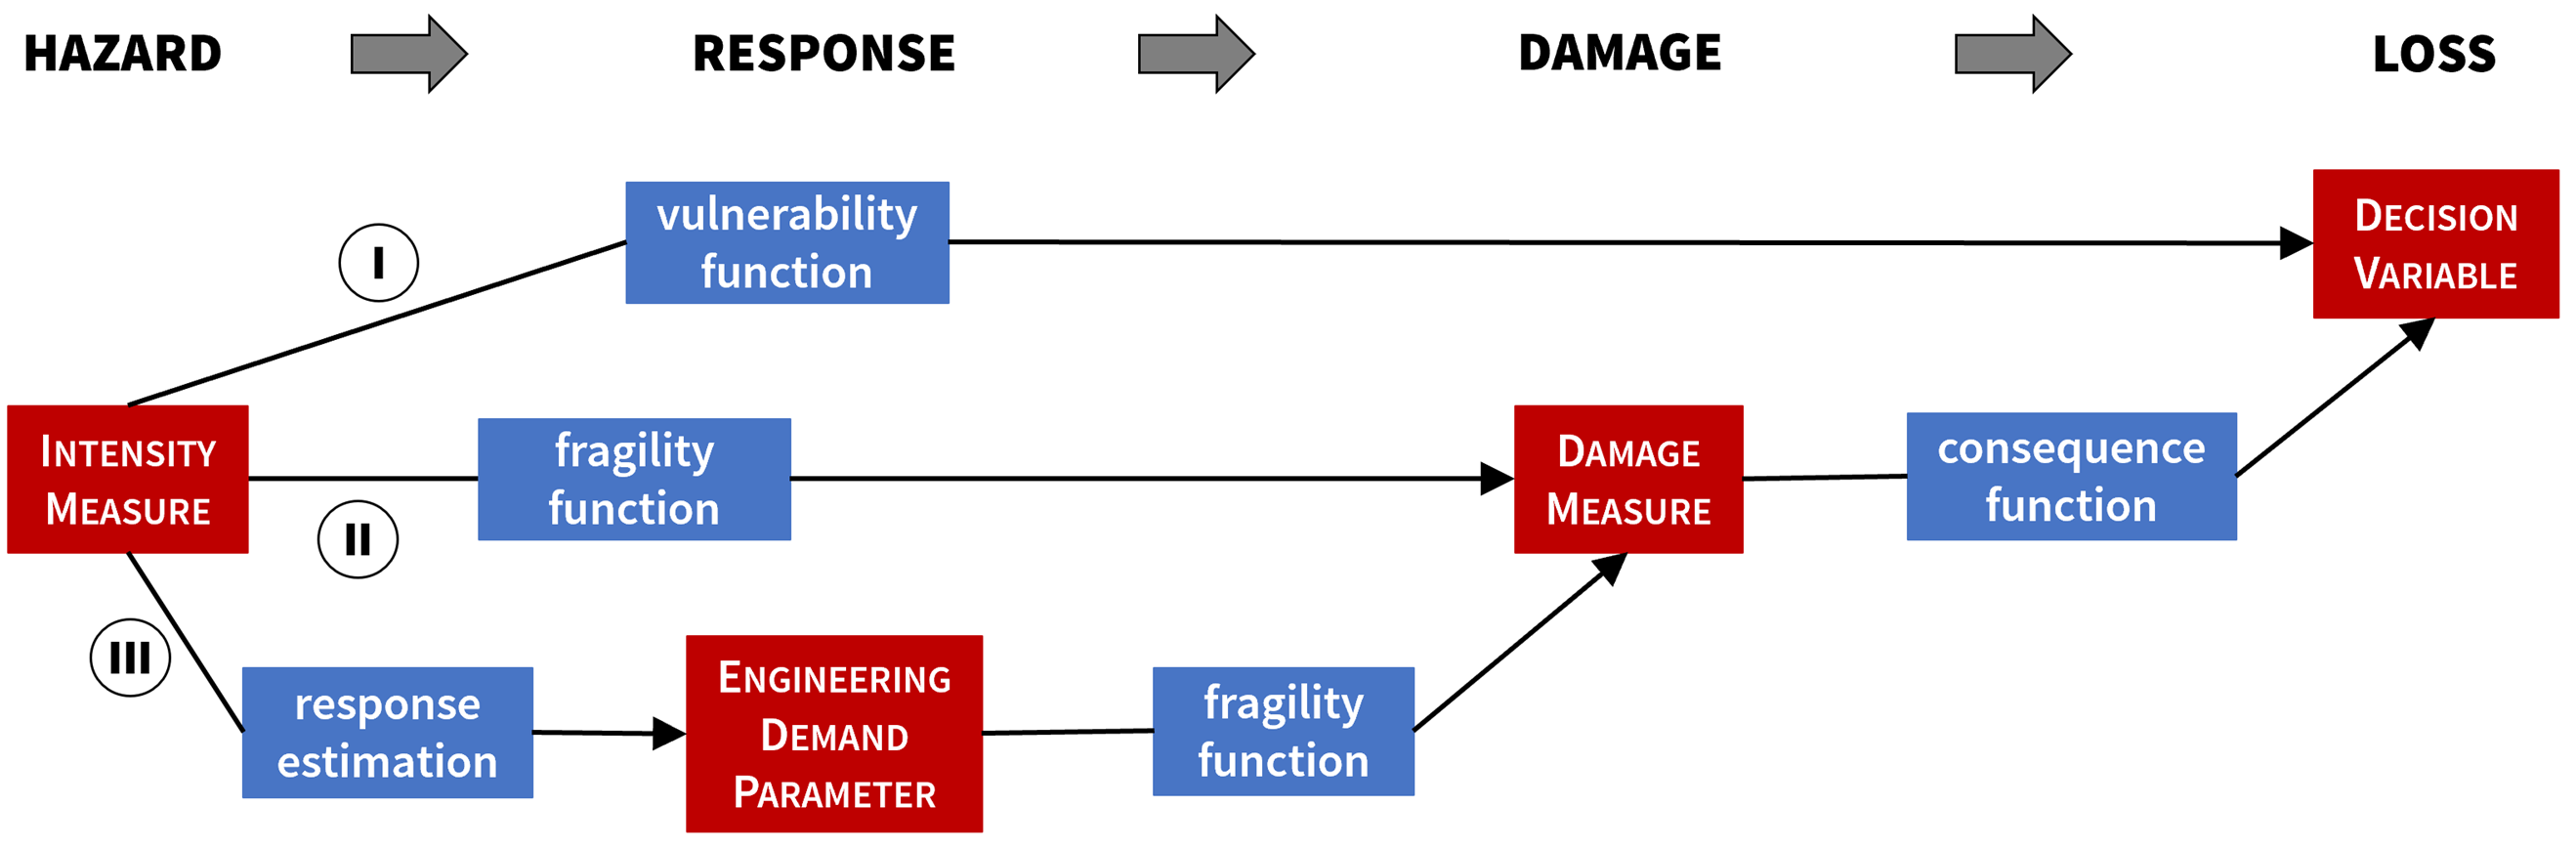
\includegraphics[width=0.9\textwidth, angle = 0]{Figures/PBEapproaches.png}
    \caption{Schematic workflows for asset performance assessment \citep{deierlein2020cloud}}
    \label{fig:perf_PBEapproaches}
\end{figure}
 
\section{Input and Output Data}
\label{sec:perf_bldg_io}

The following types of data are required to evaluate the performance of a building:

\paragraph{Hazard characterization} When the building performance is not conditioned on a particular disaster scenario, but it is evaluated considering all possible scenarios within a time period, the likelihood of each possible scenario needs to be estimated (e.g., time-based assessment in FEMA P-58 \cite{atc2018p-58-1}). The hazard curve describes the rate of exceeding various levels of an IM over the time period of interest. More information about the description of the hazard is provided in Chapter \ref{chapter:haz_shaking}.

\paragraph{Intensity Measures (IMs)} Efficient building performance assessment methods directly link intensity measures to damage measures and decision variables using fragility functions and vulnerability functions, respectively. For such methods, the inputs need to characterize the intensity of the event either through parameters of a distribution function (e.g., mean, standard deviation) or by directly providing samples of the IMs. More information about obtaining IM data is available in Chapter \ref{chapter:haz_shaking}.

\paragraph{Engineering Demand Parameters (EDPs)} High-fidelity building performance assessment uses EDPs as proxies for the detailed history of building response under a natural disaster event. EDPs shall have high correlation with the building damage of interest, and they shall be estimable with sufficiently high accuracy through numerical analysis. Estimation of EDPs first requires a building response model that is typically created in one of the environments listed in Chapter \ref{chapter:res_struct}. Second, the building model needs to be excited with loads that correspond to a particular hazard event. The inputs required for these models and analysis were described in previous parts of this report.

EDPs are extracted from the structural response simulation. Seismic performance assessment often uses peak responses at every story such as peak story drift ratios and peak floor accelerations \citep{atc2018p-58-1}. Other hazards result in different response histories and damages, and they are characterized by other EDPs, such as external pressures \citep{ouyang2020performance} or maximum inundation depth \citep{reese2011empirical}. 

\paragraph{Component characteristics} Depending on the complexity of the performance assessment method and data availability, buildings are described as a system of components or component-groups. For example, the component-group-based approach followed by HAZUS \citep{fema2011earthquaketechnical} aggregates structural components, non-structural components, and contents into three groups. The FEMA P58 method represents the other end of the spectrum; it disaggregates the building into units of components with identical behavior. The component-group-based method typically requires fewer and more generic inputs such as the type of structural system and the occupancy type to infer component behavior. The more detailed methods use the quantity, direction, and location of each component unit on each floor of the building to estimate their damage.

\paragraph{Fragility functions} Fragility functions describe the likelihood of exceeding a particular Damage State (DS) as a function of IM or EDP magnitude, (see Figure \ref{fig:perf_PBEapproaches} and \citep{baker2021seismic}). Component damages are classified into a finite number of damage states, so that each DS groups damage scenarios with similar consequences together. Fragility functions are often publicly available and there is open discussion about their improvement for the seismic performance estimation of buildings (e.g. \cite{silva2019current}). FEMA P-58 enables sophisticated analysis for seismic hazards by providing \citep{atc2012p-58} and continually revising \citep{atc2018p-58-1} a database with detailed description of more than 700 types of components. The HAZUS platform includes fragility and vulnerability functions for component-groups for various hazards, but the development of publicly-available functions that would allow more detailed assessment under wind and water hazards are a topic of active research.

\paragraph{Vulnerability and consequence functions} Vulnerability and consequence functions describe losses from a disaster as a function of its intensity and the experienced structural damage, respectively. Vulnerability functions are more efficient because they do not require information about the damages, but their estimates have more uncertainty. Vulnerability functions typically describe the consequences at a building-level (e.g., HAZUS), while consequence functions can use more detailed information (e.g., FEMA P-58) about the damage.

Direct consequences of building damage are quantified by various types of consequence functions. Each damage state has its corresponding set of consequence functions. These functions are defined by additional input data such as repair cost per component unit, affected area for calculation of injuries, or the expected time until the building can be used by its occupants. Similar to the other inputs above, these data are not exact, and the description and propagation of their uncertainty is an important part of the calculation method.

Indirect consequences and the influence of building damage on surrounding buildings and infrastructure have been considerably more difficult to model because of the scarcity of data that could be used for model calibration. Decision variables in this group include non-immediate injuries and hospital demand, displaced households and short-term shelter needs, business interruption costs, demand surge, and its influence on reconstruction cost and downtime estimates \citep{arup2013resiliencebased}.
% \newline

\paragraph{Decision variables (DVs)} Performance assessment is typically executed in a stochastic framework; the DVs are considered random, and the raw results of the assessment are at least thousands but often hundreds of thousands of samples of each variable. Therefore, interpretation and visualization of the results is an important part of the process. The majority of applications focus on mean or median values to describe central tendencies with the 10th and 90th percentiles used to illustrate the variability of results. High-performance computing and the improvement in the quality of input data create the incentive to improve estimates of the tails of the distributions and to look at the joint distribution of the variables. These analyses reveal details of complex systems that are often overlooked when focusing only at central tendencies.

\section{Modeling Approaches}
\label{sec:perf_bldg_methods}

The main assumption of the stochastic model for building performance assessment is that the uncertainty in the DVs can be estimated through the following series of independent calculations: 

\begin{itemize}
    \item describe a set of IM levels (e.g., spectral acceleration intensities) and corresponding likelihoods based on the hazard at the building location over a given time period
    \item describe the building response through EDPs given the level of the IM
    \item describe component or component-group DSs given a set of EDP realizations
    \item describe consequences using DVs given the DS of each component or component-group
    \item aggregate DVs from all components or component-groups
\end{itemize}

The calculations can be performed independently if the models used for these calculations are decoupled (e.g., the DS for two different IM levels is assumed identical if they result in identical EDPs).

The above methodology has been developed to quantify the seismic performance of buildings. It is the basis of the widely used HAZUS Earthquake Model, and it led to the development of the probabilistic seismic performance assessment framework in the Pacific Earthquake Engineering Research (PEER) Center \citep{porter2001assemblybased}. That framework, and the often cited ``triple integral,'' was the foundation of the FEMA P58 document that is considered the state-of-the-art method for seismic performance assessment of buildings today.

When it comes to building performance assessment under non-seismic hazards, the models and methods are typically more approximate. This partly stems from the lack of publicly available high-quality databases--which would drive more sophisticated model development--and from the different nature of the problem. The impact and disruption of earthquakes and hurricanes are very different in both spatial and temporal distribution, with hurricanes having a severe impact on a larger region over a longer time period. Therefore, the focus for hurricane and flood models have always tended to be more regional where capturing the detailed response of individual structures receives less attention.

\section{Research Gaps and Needs}
\label{sec:perf_bldg_gaps}

Tom O'Rourke: there is a need to better understand urban seismic vulnerability, the interaction between buildings and also between buildings and the other components of the built environment.

\section{Software and Systems}
\label{sec:perf_bldg_tools}

The following is a list of software that provides features required for state-of-the-art research in building performance assessment:
% \newline

\paragraph{CAPRA} Development of the Comprehensive Approach to Probabilistic Risk Assessment (\citeprgm{CAPRA}) platform was initially supported by the World Bank and the Inter-American Development Bank; it has been managed by Uniandes (Universidad de los Andes in Colombia) since 2017. CAPRA is designed to become a multi-hazard framework based on several modules that handle different tasks of the risk assessment workflow. The currently available modules allow risk assessment using vulnerability functions for several types of hazards (e.g., earthquake, hurricane, and flood). The open source CAPRA framework uses Visual Basic .NET and provides applications in a Windows environment.
% \newline

\paragraph{MAEViz} 
Developed by the Mid-America Earthquake Center (MAE), \citeprgm{MAEViz} is based on the HAZUS methodology for scenario risk assessment and it allows users to write their own extensions. Through these added modules, its functionality is not limited to building performance assessment and allows analysis of infrastructure and lifeline performance as well as indirect consequences in the region. It uses a Windows-based application with a user interface to guide the user through the analysis. MAEViz is open source and has been integrated into several platforms in the US [e.g., ERGO, mHARP] and in Europe [e.g., SYNER-G \citep{pitilakis2014synerg} and HAZturk \citep{karaman2008earthquake}].

\paragraph{HAZUS 4.2} The FEMA-supported \citeprgm{HAZUS4x2} tool was already introduced in Section 1.1. The damage and loss assessment modules in HAZUS use the component-group-based approach and categorize components into structural, non-structural, and content groups. The methodology provides estimates of direct and indirect consequences of damage. Its efficiency allows it to be scaled to a regional level without having to resort to HPC.
% \newline

\paragraph{OpenQuake} 
\citeprgm{OpenQuake} is developed and maintained by The GEM Foundation. The source code is written in Python, open source, and publicly available at a github repository. OpenQuake provides a platform to perform regional disaster risk assessment. The Hazard part of the library has already been mentioned in Section 1.1. The Risk part of the library performs a component-group based performance assessment that is similar to the approach by HAZUS. Input data for the platform is collected and made publicly available in an online repository at platform.openquake.org. Currently, OpenQuake leans heavily towards seismic hazard and risk assessment, but there are developments towards flood impacts, and the framework is sufficiently flexible to allow other extensions as well.

\paragraph{OpenSLAT} The Open Seismic Loss Assessment Tool (\citeprgm{OpenSLAT})is an open-source library developed at the University of Canterbury written in C++ and Python. It is publicly available and allows researchers to use the developed functions in their preferred environment. It implements the Magnitude-oriented Adaptive Quadrature (MAQ) algorithm developed by \cite{bradley2010efficient} to efficiently solve the integrals involved in PBE calculations.


\paragraph{PACT} The Performance Assessment Calculation Tool (\citeprgm{PACT}), developed by the Applied Technology Council (ATC) is a publicly available software that implements the performance assessment methodology in the FEMA P58 document \citep{atc2018p-58-2}. It is designed to describe the performance of a single building, not a region with a collection of buildings. The software is controlled by a GUI and is available for the Windows platform only. It does not perform hazard and structural response calculations, but rather requires the results of those calculations as inputs. All fragility and consequence functions developed in the FEMA P58 project are conveniently available in PACT.

\paragraph{PBE Application} The Performance Based Engineering Application (\citeprgm{PBE}) has been developed by the NHERI SimCenter to provide a convenient GUI-based tool for researchers interested in performance assessment \citep{mckenna2018performance}. The GUI provides access to the versatile PBE workflow developed at the SimCenter and allows users to choose the tools and methods they wish to use for hazard estimation, response simulation, and loss assessment. The application facilitates the use of high-performance computing resources by providing a built-in connection to the Stampede 2 supercomputer at UT Austin through DesignSafe \citep{rathje2017designsafe}.

Currently, the application is limited to seismic hazards, with wind and water hazards features under development. Seismic hazard assessment uses OpenSHA (see Section 1.1), response estimation uses OpenSEES (see Section 2.1), and loss assessment uses PELICUN (see below) to perform the calculations. Future versions will expand the set of available tools in the application.
% \newline

\paragraph{PELICUN} The Probabilistic Estimation of Losses, Injuries, and Community resilience Under Natural Disasters tool (\citeprgm{PELICUN}) is an open-source Python library developed by the SimCenter. It is publicly available at the SimCenter github repository (Zsarnóczay, 2018). The library is designed to provide a versatile, platform-independent and transparent loss-assessment tool for the research community. It is based on a stochastic loss model that allows detailed component-based as well as simplified component-group-based loss assessment. The current version implements the scenario-based assessment from the FEMA P58 methodology. The HAZUS methodology for earthquakes and the time-based assessment option are under development. The library allows researchers to work in their preferred environment and call its functions to perform loss assessment. PELICUN is used in the applications developed by the SimCenter for performance assessment.
% \newline

\paragraph{SP3} The Seismic Performance Prediction Program (\citeprgm{SP3}) is proprietary software developed by the Haselton Baker Risk Group. It is widely considered the most reliable implementation of the FEMA P58 methodology and ARUP's REDi framework for downtime estimation; it is used by practitioners and researchers. Besides the high-quality implementation, the tool is also bundled with valuable data that facilitates building response estimation, and damage and loss assessment. The tool can be accessed through a web-based interface that guides the user through the steps of performance assessment. Researchers with programming skills can use it in batch mode that enables more powerful analyses. The calculations run on Amazon EC2 servers, which allow users to run complex, demanding analyses within a reasonable timeframe.

